\documentclass[UTF8,zihao=false,fontset=fandol]{ctexart}

\usepackage[paperwidth=760mm,paperheight=1140mm,margin=0mm]{geometry}
\usepackage{fontspec}
\usepackage{graphicx}
\usepackage{xcolor}
\usepackage{tikz}
\usepackage{tabularx}
\usepackage{booktabs}
\usepackage{listings}
\usepackage{amsmath,amssymb,mathtools}
\usepackage{enumitem}

\pagestyle{empty}
\setlength{\parindent}{0pt}
\setlength{\parskip}{0.45mm}
\linespread{1.0}

\IfFontExistsTF{TeX Gyre Heros}{\setsansfont{TeX Gyre Heros}}{}
\IfFontExistsTF{TeX Gyre Termes}{\setmainfont{TeX Gyre Termes}}{}
\IfFontExistsTF{Menlo}{\setmonofont{Menlo}}{}

\definecolor{ink}{HTML}{13203A}
\definecolor{muted}{HTML}{5B667E}
\definecolor{rule}{HTML}{D7DAE3}
\definecolor{soft}{HTML}{F7F8FA}
\definecolor{hot}{HTML}{C0392B}
\definecolor{cool}{HTML}{2C6E8F}
\definecolor{greenx}{HTML}{2E7D32}

\newcommand{\bodyfont}{\fontsize{14.2pt}{17.4pt}\selectfont}
\newcommand{\smallbody}{\fontsize{11.8pt}{14.2pt}\selectfont}
\newcommand{\tinybody}{\fontsize{9.2pt}{10.8pt}\selectfont}
\newcommand{\sectionfont}{\fontsize{19.2pt}{23pt}\selectfont\bfseries}
\newcommand{\subfont}{\fontsize{13.4pt}{16pt}\selectfont\bfseries}

\newcommand{\sect}[2]{%
  \vspace{2.2mm}
  {\sectionfont\textcolor{hot}{\texttt{#1}}\hspace{3mm}#2}\par
  \vspace{0.8mm}\textcolor{rule}{\rule{\linewidth}{0.65pt}}\vspace{0.5mm}
}

\newcommand{\subsect}[1]{%
  \vspace{0.8mm}{\subfont #1}\par\vspace{0.3mm}
}

\newcommand{\algline}[3]{%
  \par\noindent
  \makebox[5mm][r]{\tinybody\ttfamily\textcolor{muted}{#1}}\hspace{2mm}%
  \begin{minipage}[t]{\dimexpr\linewidth-8mm}
    \smallbody #2\hfill{\tinybody\itshape\textcolor{muted}{#3}}
  \end{minipage}
}

\lstdefinestyle{posterpython}{
  language=Python,
  basicstyle=\ttfamily\fontsize{8.9pt}{10.6pt}\selectfont\color{ink},
  backgroundcolor=\color{white},
  keywordstyle=\color{cool}\bfseries,
  stringstyle=\color{greenx!80!black},
  commentstyle=\color{muted},
  showstringspaces=false,
  frame=none,
  rulecolor=\color{rule},
  breaklines=true,
  columns=fullflexible,
  keepspaces=true,
  xleftmargin=0mm,
  xrightmargin=0mm,
  aboveskip=1mm,
  belowskip=0mm
}

\begin{document}

\begin{tikzpicture}[remember picture,overlay]
  \node[anchor=south west,inner sep=0pt] at (current page.south west)
    {
\includegraphics[width=\paperwidth,height=\paperheight]{poster_assets/poster_bg.jpg}};
  \node[anchor=north,align=center,text width=700mm,inner sep=0pt]
    at ([yshift=-100mm]current page.north) {%
      {\sffamily\bfseries\fontsize{43pt}{50pt}\selectfont\color{white}
      \mbox{FEP-RLVE: 用\textcolor{yellow!72!white}{期望自由能}选择训练难度}}\par
      \vspace{2mm}
      {\sffamily\bfseries\fontsize{23pt}{28pt}\selectfont\color{white!94}
      Curriculum by Active Inference for Verifiable Environments}\par
      \vspace{5mm}
      {\sffamily\itshape\fontsize{15.2pt}{19pt}\selectfont\color{white!88}
      把 RLVE 的 ``$\mathrm{acc}\ge0.9$ 升难'' 启发式, 换成 active-inference 的行动选择}\par
      \vspace{4mm}
      {\ttfamily\fontsize{10.8pt}{13pt}\selectfont\color{white!78}
      姓名 / 学号 \quad RL with Env Scaling \quad ProRL-1.5B-v2 \quad 单卡 H200}
    };

  \draw[color=rule,line width=0.9pt]
    ([xshift=380mm,yshift=-282mm]current page.north west)
    -- ([xshift=380mm,yshift=-1038mm]current page.north west);

  \node[anchor=north west,inner sep=0pt,text width=344mm]
    at ([xshift=22mm,yshift=-276mm]current page.north west) {%
      \begin{minipage}{344mm}
      \bodyfont\color{ink}
      \sect{01}{问题与核心目标}
      GRPO/DAPO 以一组 $K$ 个 rollout 为单位更新。若一组全对或全错, 组内奖励方差为零, 优势项为零, 该 prompt 基本不产生有效 policy gradient。
      \[
        U_K(p)=\Pr(0<k<K)=1-p^K-(1-p)^K,\qquad
        p^\star=\arg\max_p U_K(p)=\tfrac12 .
      \]
      因此课程控制的目标不是让模型尽快达到高准确率, 而是让训练样本成功率贴近 $p=0.5$ 的最大信号带。以 $K=8$ 为例,
      $U_8(0.9)\approx0.57$, 而 $U_8(0.5)\approx0.99$。

      \vspace{2mm}
      \begin{tabularx}{\linewidth}{>{\bfseries\color{cool}}p{38mm}X}
      太难 & $p\to0$, 奖励稀疏, 只有少数 rollout 给信号\\
      太易 & $p\to1$, 组内方差消失, 优势退化\\
      合适 & $p\approx0.5$, 正负样本混合, policy gradient 最强\\
      \end{tabularx}

      \sect{02}{自由能建模}
      把 ``选择训练难度'' 看成行动选择: 训练器维护每个环境 $e$ 的能力信念 $q_e(s)$, 观测 verifier 的对/错反馈 $o\in\{0,1\}$, 再选择下一步难度 $d$。

      \[
        \mathcal F[q]
        =D_{\rm KL}\!\left(q(s)\Vert p(s\mid o)\right)-\log p(o)
      \]
      最小化变分自由能等价于用观测更新能力信念。行动侧使用期望自由能:
      \[
        G_e(d)=\lambda_{\rm sig}\big[-\log U_K(\hat p_e(d))\big]
        -\lambda_{\rm info}I_q(s_e;o\mid d)
        +\lambda_{\rm cost}C_e(d)
      \]
      \[
        \pi(d\mid e)=
        \frac{\exp(-G_e(d)/T)}
        {\sum_{d'}\exp(-G_e(d')/T)},\qquad
        \hat p_e(d)=\mathbb E_{s\sim q_e}\sigma(a(s-d)).
      \]

      \begin{itemize}[leftmargin=6mm,itemsep=0.5mm,topsep=0.5mm]
        \item \textcolor{hot}{实用项}: $-\log U_K(\hat p)$ 惩罚全对/全错的低信号区域。
        \item \textcolor{cool}{认知项}: $I_q(s_e;o\mid d)$ 鼓励选择最能缩小不确定性的难度。
        \item $T$ 控制探索强度; $T\to0$ 接近贪心, $T\to\infty$ 接近均匀探索。
      \end{itemize}

      \vspace{1mm}
      RLVE 的 ``$\mathrm{acc}\ge0.9\Rightarrow d\leftarrow d+1$'' 是硬阈值特例; FEP-RLVE 把它改成可推导、可消融、可升可降的连续目标。
      \end{minipage}
    };

  \node[anchor=north west,inner sep=0pt,text width=344mm]
    at ([xshift=394mm,yshift=-276mm]current page.north west) {%
      \begin{minipage}{344mm}
      \bodyfont\color{ink}
      \sect{03}{算法与代码}
      \begin{minipage}[t]{0.49\linewidth}
      \smallbody
      \textbf{Algorithm 1 \quad RLVE}\par
      \tinybody\itshape Require: $\mathcal E$, $\tau=0.9$, $\Delta$\par
      \vspace{0.8mm}
      \algline{1}{\textbf{for} $e\in\mathcal E$: $h_e\leftarrow0$}{难度上界}
      \algline{2}{采样 $e$; $d\sim\mathrm{Unif}\{h_e-\Delta,\ldots,h_e\}$}{邻域}
      \algline{3}{rollouts $\leftarrow\pi_\theta$; $r_j\leftarrow\mathrm{verify}(y_j)$}{}
      \algline{4}{$\theta\leftarrow\mathrm{GRPO}(\theta;\{r_j\}_{j=1}^K)$}{}
      \algline{5}{若 $\widehat{\mathrm{acc}}_e\ge\tau$, $h_e\leftarrow h_e+1$}{只升}
      \end{minipage}\hfill
      \begin{minipage}[t]{0.49\linewidth}
      \smallbody
      \textbf{Algorithm 2 \quad FEP-RLVE}\par
      \tinybody\itshape Require: $q_e(s)$, $\lambda$, $T$, $K$\par
      \vspace{0.8mm}
      \algline{1}{采样环境 $e$}{}
      \algline{2}{\textbf{for} $d=d_{\min},\ldots,d_{\max}$}{估 EFE}
      \algline{3}{\hspace{6mm}$\hat p_d\leftarrow\sum_s q_e(s)\sigma(a(s-d))$}{}
      \algline{4}{\hspace{6mm}$U_d\leftarrow1-\hat p_d^K-(1-\hat p_d)^K$}{}
      \algline{5}{\hspace{6mm}$I_d\leftarrow H_b(\hat p_d)-\sum_s q_e(s)H_b(\sigma(a(s-d)))$}{}
      \algline{6}{\hspace{6mm}$G_d\leftarrow\lambda_{\rm sig}(-\log U_d)-\lambda_{\rm info}I_d+\lambda_{\rm cost}C_d$}{}
      \algline{7}{$d\sim\mathrm{softmax}(-G/T)$; 更新 $q_e(s)$}{可升降}
      \end{minipage}

      \vspace{1mm}
      \begin{lstlisting}[style=posterpython]
def signal(self, d):
    return U_K(self.p_hat(d), self.K)

def pragmatic(self, d):
    return -math.log(max(self.signal(d), 1e-12))

def info_gain(self, d):
    pbar = self.p_hat(d)
    cond = sum(qi * _Hb(self._p(s, d))
               for qi, s in zip(self.q, self.s_grid))
    return _Hb(pbar) - cond

def G(self, d):
    return (self.l_sig * self.pragmatic(d)
            - self.l_info * self.info_gain(d)
            + self.l_cost * self.C(d))
      \end{lstlisting}

      \smallbody
      \texttt{rlve\_repro/active\_inference\_controller.py} 实现 EFE;
      \texttt{active\_inference\_manager.py} 在 \texttt{generate\_problem()} 中采样 $d$, 在 \texttt{update()} 中用 verifier 结果更新 $q_e(s)$。

      \sect{04}{实验结果与结论}
      \begin{minipage}[t]{0.49\linewidth}
        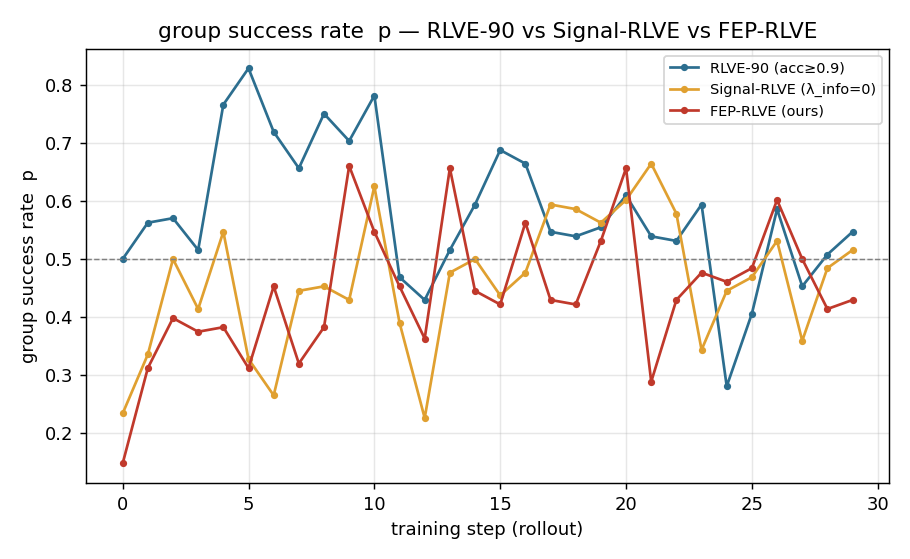
\includegraphics[width=\linewidth]{results/figures/success_rate.png}
        \tinybody 图 1. 成功率贴近 $p=0.5$ 信号最优带。
      \end{minipage}\hfill
      \begin{minipage}[t]{0.49\linewidth}
        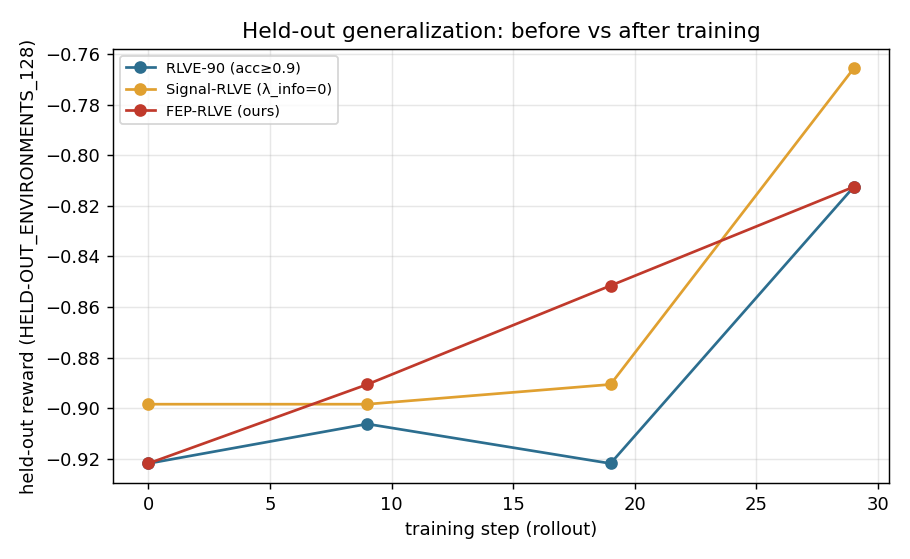
\includegraphics[width=\linewidth]{results/figures/heldout.png}
        \tinybody 图 2. held-out reward 三臂均提升。
      \end{minipage}

      \vspace{1.2mm}
      \begin{tabularx}{\linewidth}{lccc}
      \toprule
      臂 & 成功率 & $U_K$ & held-out 前到后\\
      \midrule
      RLVE-90 & 0.58 & 0.962 & $-0.92\to-0.81$\\
      Signal-RLVE & 0.46 & 0.974 & $-0.90\to\mathbf{-0.77}$\\
      \textcolor{hot}{\bfseries FEP-RLVE} & 0.44 & 0.970 & $-0.92\to-0.81$\\
      \bottomrule
      \end{tabularx}

      \vspace{1mm}
      Signal 终值最好, FEP 提升更单调。主要贡献是把启发式升难改成可解释的 EFE 目标; 主要边界是小规模实验增益温和, 且单标量能力假设仍需更复杂环境验证。
      \end{minipage}
    };

  \node[anchor=south,align=center,text width=700mm,font=\ttfamily\fontsize{10.5pt}{12.5pt}\selectfont,text=white]
    at ([yshift=18mm]current page.south)
    {code: github.com/0xLian117/RLproj \quad baseline: RLVE (arXiv:2511.07317) \quad related: SCALER (arXiv:2601.04809) \quad free energy: Friston et al.};
\end{tikzpicture}

\null

\end{document}
